
\subsection{Timeline}

Timestamps are used to assign an event a unique moment. With the help of these timestamps a timeline can be created. In this timeline you can see which action was done to an object at a specific time and which action followed after a specific action. The timeline also  represents, what kind of action (created, modified, accessed) had taken place. You can find the timestamps in different metadata of the system. Timestamps can be found in different metadata like in file system, application, log data and many other data. Metadata are data about data and are usually stored with the digital object. In different digital objects you can find different metadata. For example in a taken photo you find other metadata as in a word document. In a photo you find information like the ISO value and exposure time which you can not find in a word document. The important metadata for the timeline are the different times. These times are called MACtimes. Advertised the three letter means the following. M stands for the modified time (mtime), a  stands for the accessed time (atime) and c stands for the changed time (ctime). It can happen that all of these times show the same time. The accessed time means the time at which the file was the last time read. The modified time means the time at which the content of the file was changed. The changed time means the time at which the metadata of a file was changed. For example a file got another permission or owner. NTFS the file system of current Windows versions owns a fourth time. This time is called born time (btime). This is the time at which the object was created. The born time is in Linux (Ext2, Ext3) not available. In Table~\ref{fig:Mactimes} you can see the meaning of MACtimes in different file systems. In figure~\ref{fig:timeline} you see a created timeline. This timeline was created for the project and shows chronologically what a criminal did. At first the criminal loaded files from the internet with illegal content. Then a truecrypt-container (setup.exe) was created and changed. Changed means in this context that the container were probably added with data. After that the criminal accessed to these data and read these data. Later, it can be seen, two other truecrypt-container were created. We got the various timestamps with the help of the tool “Redline”. Using a timeline is used to reconstructed in what order the offender went on and which objects were created, accessed or modified.

\begin{table}[h]

\begin{tabular}{c|c|c|c|c}
	File System & modified & accessed & changed & birth \\
	\hline \hline
	Ext2/3 & modified & accessed & changed & N/A \\
	\hline
	FAT & written & accessed & N/A & created \\
	\hline
	NTFS & file modified & accessed & MFT modified & created \\
	\hline
	UFS & modified & accessed & changed & N/A \\

\end{tabular}

\caption{Mactimes}
\label{fig:Mactimes}
\end{table}

There are also problems with the analysis of the timeline. The timestamps are faulty if the computer which is examined is in a different time zone. One problem which exists in the NTFS file system is that it can take until one hour to update the access time after it was accessed. Furthermore criminal can change the MACtimes with help of software. One of these programs which can change the timestamps is named “BulkFileChanger”. BulkFileChanger can modify the created, modified and accessed time. Thus a criminal could disorient a digital researcher. All of these issues need to be considered in order to get an accurate result. One problem more which exists, sometimes it is difficult to know if an object was accessed by a application or a person. 

There are important hints for a digital researcher. These hints can tell a digital researcher what happened with a file. The digital researcher recognizes through the combination of Mactimes which action happened to a file, e. g. if the modified time is before the created time, then the file was copied from one system or moved from one partition to another partition. There are more of these methods and that can be written in the paper "http://www.cs.hku.hk/cisc/forensics/papers/RuleOfTime.pdf".









\begin{figure}[tbph]
	\centering
		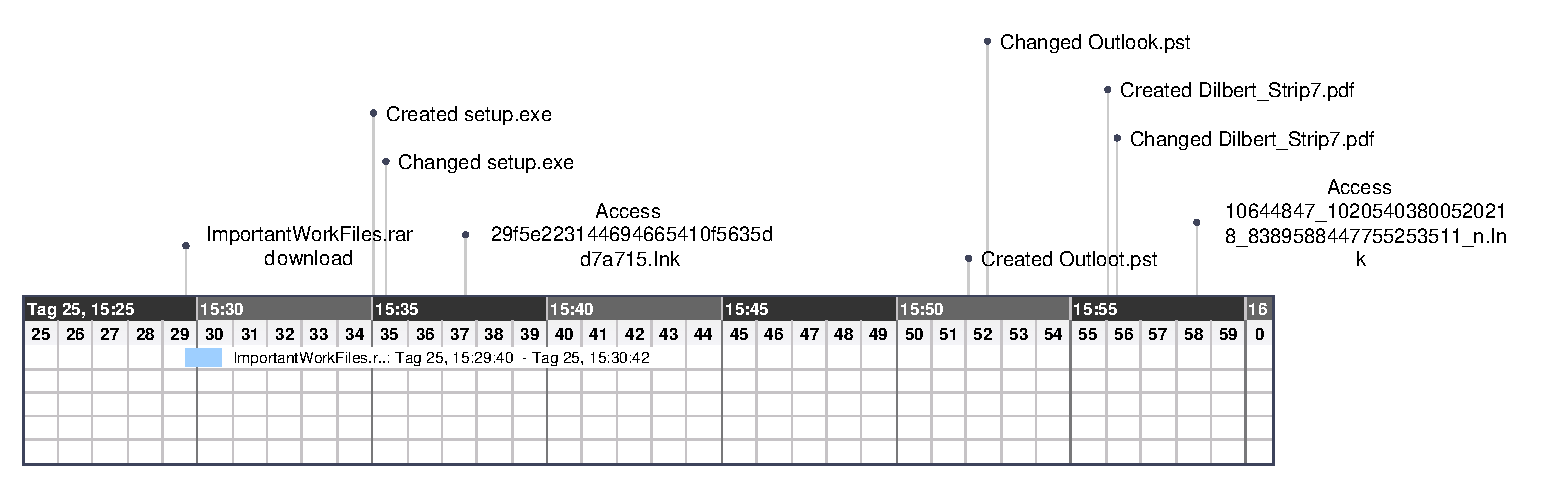
\includegraphics[width=\textwidth]{graphics/Timeline.pdf} 	
	\caption{Timeline}
	\label{fig:timeline}
\end{figure}






